\documentclass[9pt]{article}
\usepackage[top=3cm, bottom=3cm, outer=3cm, inner=3cm]{geometry}
\usepackage{multicol}
\usepackage{graphicx}
\usepackage{url}
\usepackage{hyperref}
\usepackage{array}
\newcolumntype{x}[1]{>{\centering\arraybackslash\hspace{0pt}}p{#1}}
\usepackage{natbib}
\usepackage{multirow}
\usepackage[normalem]{ulem}
\useunder{\uline}{\ul}{}
\usepackage{listings}
\lstdefinestyle{ascii-tree}{
	literate={├}{|}1 {─}{--}1 {└}{+}1 
}
\lstset{basicstyle=\ttfamily,
	showstringspaces=false,
	commentstyle=\color{red},
	keywordstyle=\color{blue}
}
\usepackage{caption}
\usepackage{subcaption}
\usepackage{float}
\usepackage{array}
\usepackage{longtable}
\usepackage{tabularx}
\usepackage{adjustbox}
\usepackage[table]{xcolor}% http://ctan.org/pkg/xcolor
\usepackage{blindtext}
\renewcommand{\familydefault}{\sfdefault}
\usepackage{geometry}
\geometry{
	a4paper,
	total={190mm,257mm},
	left=10mm,
	top=20mm,
}
\newcolumntype{M}[1]{>{\centering\arraybackslash}m{#1}}
\newcolumntype{N}{@{}m{0pt}@{}}
%%%%%%%%%%%%%%%%%%%%%%%%%%%%%%%%%%%%%%%%%%%%%%%%%%%%%%%%%%%%%%%%%%%%%%%%%%%%
%%%%%%%%%%%%%%%%%%%%%%%%%%%%%%%%%%%%%%%%%%%%%%%%%%%%%%%%%%%%%%%%%%%%%%%%%%%%
\newcommand{\itemCourse}{Estructura de Datos y Algoritmos}
\newcommand{\itemUniversity}{Universidad Nacional de San Agustín de Arequipa}
\newcommand{\itemFaculty}{Facultad de Ingeniería de Producción y Servicios}
\newcommand{\itemDepartment}{Departamento Académico de Ingeniería de Sistemas e Informática}
\newcommand{\itemSchool}{Escuela Profesional de Ingeniería de Sistemas}
\newcommand{\itemPracticeNumber}{06}
\newcommand{\itemTheme}{Arbol AVL}
%%%%%%%%%%%%%%%%%%%%%%%%%%%%%%%%%%%%%%%%%%%%%%%%%%%%%%%%%%%%%%%%%%%%%%%%%%%%
%%%%%%%%%%%%%%%%%%%%%%%%%%%%%%%%%%%%%%%%%%%%%%%%%%%%%%%%%%%%%%%%%%%%%%%%%%%%
\usepackage[english,spanish]{babel}
\usepackage[utf8]{inputenc}
\AtBeginDocument{\selectlanguage{spanish}}
\renewcommand{\figurename}{Figura}
\renewcommand{\refname}{Referencias}
\renewcommand{\tablename}{Tabla} %esto no funciona cuando se usa babel
\AtBeginDocument{%
	\renewcommand\tablename{Tabla}
}
\usepackage{fancyhdr}
\pagestyle{fancy}
\fancyhf{}
\setlength{\headheight}{30pt}
\renewcommand{\headrulewidth}{1pt}
\renewcommand{\footrulewidth}{1pt}
\fancyhead[L]{\raisebox{-0.2\height}{
\includegraphics[width=3cm]{img/logo_episunsa.png}}}
\fancyhead[C]{\fontsize{7}{7}\selectfont	\itemUniversity \\ \itemFaculty \\ \itemDepartment \\ \itemSchool \\ \textbf{\itemCourse}}
\fancyhead[R]{\raisebox{-0.2\height}{
\includegraphics[width=1.2cm]{img/logo_abet}}}
\fancyfoot[C]{\itemCourse}
\fancyfoot[R]{Página \thepage}
\usepackage{listings}
\usepackage{color, colortbl}
\definecolor{dkgreen}{rgb}{0,0.6,0}
\definecolor{gray}{rgb}{0.5,0.5,0.5}
\definecolor{mauve}{rgb}{0.58,0,0.82}
\definecolor{codebackground}{rgb}{0.95, 0.95, 0.92}
\definecolor{tablebackground}{rgb}{0.8, 0, 0}
\lstset{frame=tb,
	language=bash,
	aboveskip=3mm,
	belowskip=3mm,
	showstringspaces=false,
	columns=flexible,
	basicstyle={\small\ttfamily},
	numbers=none,
	numberstyle=\tiny\color{gray},
	keywordstyle=\color{blue},
	commentstyle=\color{dkgreen},
	stringstyle=\color{mauve},
	breaklines=true,
	breakatwhitespace=true,
	tabsize=3,
	backgroundcolor= \color{codebackground},
}
\begin{document}
	
	\vspace*{10px}
	
	\begin{center}	
		\fontsize{17}{17} \textbf{ Informe de Laboratorio \itemPracticeNumber}
	\end{center}
	\centerline{\textbf{\Large Tema: \itemTheme}}
	%%%%%%%%%%%%%%%%%%%%%%%%%%%%%%%%%%%%%%%%%%%%%%%%%%%%%%%%%%%%%%%%%%%%%%%%%%%%
	\begin{adjustbox}{width=\textwidth}
		\begin{tabularx}{\textwidth} {
				| >{\raggedright\arraybackslash}X 
				| >{\raggedright\arraybackslash}X 
				| >{\raggedright\arraybackslash}X 
				| >{\raggedright\arraybackslash}X
				| >{\raggedright\arraybackslash}X
				| >{\raggedright\arraybackslash}X |}
			\hline
			\rowcolor{tablebackground}
			\multicolumn{6}{ | c | }{\color{white}\textbf{INFORMACIÓN BÁSICA}} \\
			\hline
			\textbf{ASIGNATURA:}& \multicolumn{5}{ | l | }{\textbf{\itemCourse}} \\
			\hline
			\textbf{TÍTULO DEL TRABAJO:} & \multicolumn{5}{ | l | }{Tries} \\
			\hline
			\textbf{NÚMERO DE TRABAJO:}& 06 & \textbf{AÑO LECTIVO:} & 2023-A & \textbf{NRO. SEMESTRE:} & III \\
			\hline
			\textbf{FECHA DE PRESENTACIÓN:} & 23/07/23 &\textbf{HORA DE PRESENTACIÓN:}& \multicolumn{3}{ | l | }{23:59} \\
			\hline
			\multicolumn{4}{ | l | }{\textbf{INTEGRANTE (s)}} & \textbf{NOTA (0-20)} & \\
			\hline
			\multicolumn{6}{ | l | }{\textbf{Hidalgo Chinchay, Paulo Andre}}\\
			\multicolumn{6}{ | l | }{\textbf{Betanzos Rosas, Taylor Anthony}}\\
			\multicolumn{6}{ | l | }{\textbf{Villafuerte Ccapira Frank Alexis}} \\
			\hline
			\multicolumn{6}{ | l | }{\textbf{DOCENTE(s):}} \\
			\multicolumn{6}{ | l | }{Mg. Edith Giovanna Cano Mamani} \\
			\hline
		\end{tabularx}
	\end{adjustbox}
	
	%%%%%%%%%%%%%%%%%%%%%%%%
	\begin{longtable}{|p{15cm}|}
		\caption{Mi tabla extendida}\\
		\hline 
		\rowcolor{tablebackground}
		\color{white}\textbf{INTRODUCCIÓN}  \\
		\hline 
		\textbf{Se implementaran los diferentes metodos con los que cuentan los Tries
		como son la insercion, busqueda y eliminacion, con la finalidad de crear un programa
		que permita ingresar palabras, buscarlas y reemplazarlas.}  \\
		\hline 
		%%%%%%%%%%%%
		\rowcolor{tablebackground}
		\color{white}\textbf{MARCO CONCEPTUAL}  \\
		\hline 
		\textbf{Un trie es una estructura de datos de tipo árbol que permite
		 la recuperación de información.
		  La información almacenada en un trie es un conjunto de claves, donde 
		  una clave es una secuencia de símbolos pertenecientes a un alfabeto. 
		  Las claves son almacenadas en las hojas del árbol y los nodos internos 
		  son pasarelas para guiar la búsqueda. El árbol se estructura de forma 
		  que cada letra de la clave se sitúa en un nodo de forma que los hijos
		de un nodo representan las distintas posibilidades de símbolos diferentes
		que pueden continuar al símbolo representado por el nodo padre. Por tanto 
		la búsqueda en un trie se hace de forma similar a como se hacen las búsquedas 
		en un diccionario[1]}  \\		
		\hline 
		%%%%%%%%%%%%
		\rowcolor{tablebackground}
		\color{white}\textbf{SOLUCIONES Y PRUEBAS}  \\
		\hline
		\textbf{ Para el metodo insert se iteraba con un for letra por letra de la palabra a insertar
		para luego obtener su valor en el codigo ACSSI, con el valor resultante con
		se veia si el hijo del TrieNode actual era nulo, si era nulo se creaba un nuevo TrieNode
		con un valor de endOfWord en falso, hasta llegar a la penultima letra de la palabra, en la cual se terminaba 
		el for y se creaba un nuevo TrieNode con el valor de endOfWord en verdadero.}\\
		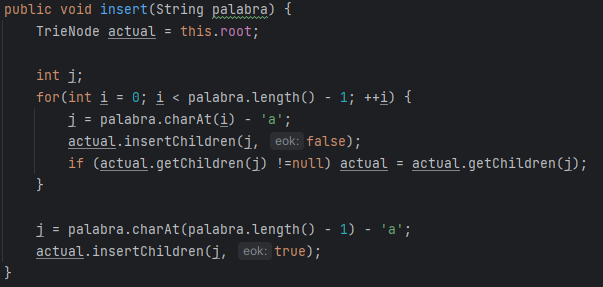
\includegraphics[width=0.85\textwidth,keepaspectratio]{img/insert.png}\\


		\textbf{Para el metodo search se iteraba caracter por caracter de la palabra buscada
		al ifual que en el metodo insert, sin embargo, si aqui el hijo del nodo actual era nulo
		retornaba false y si no continuaba con el ciclo hasta la penultima letra. La ultima letra
		a parte de existir debia tambien cumplir en ser endOfWord retornando asi la union de estos
		2 valores.}\\
		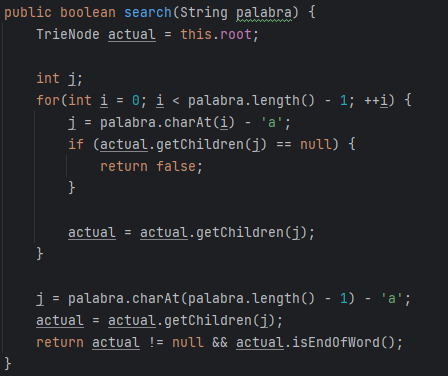
\includegraphics[width=0.85\textwidth,keepaspectratio]{img/search.png}\\

		\textbf{ El método delete sirve para eliminar una palabra el cual era un metodo recursivo
		que retornaba un boolean, lo cual permitia saber si se debe o no eliminar un TrieNode
		con esto se eliminaba de la ultima letra hasta la 1ra, en caso no hubiera un endOfWord
		en el camino, en caso fuera asi, dejaba de eliminar.}\\
		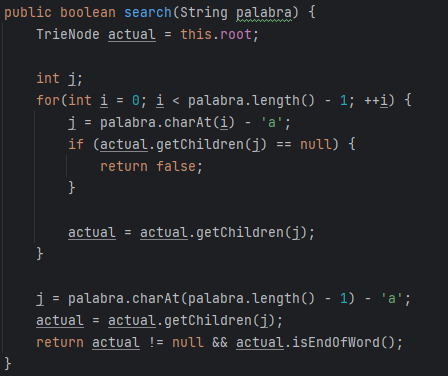
\includegraphics[width=0.85\textwidth,keepaspectratio]{img/search.png}\\
		\textbf{Para obtener el máximo solo se retorna la raíz, ya que es un AVL máximo.		}\\
		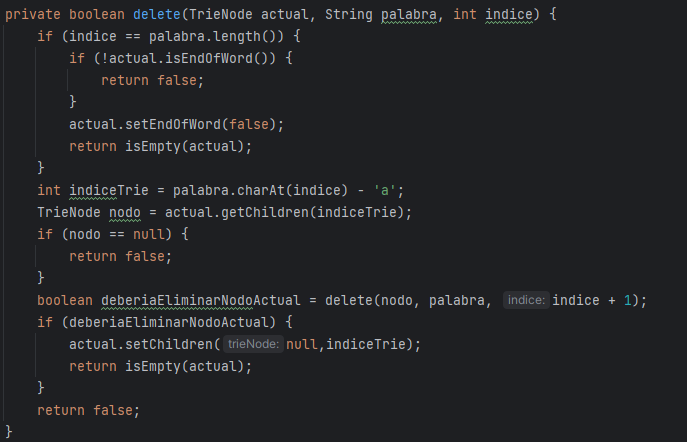
\includegraphics[width=0.6\textwidth,keepaspectratio]{img/delete.png}\\
		\textbf{El metodo replace, sirve para reemplazar un palabra por otra,
		por lo cual elimina una palabra y pone a la otra en su lugar, para ello
		utiliza los metodos delete e insert respectivamente.}  \\
		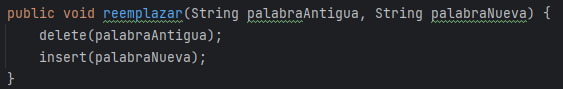
\includegraphics[width=0.8\textwidth,keepaspectratio]{img/replace.png}\\
		\textbf{Ejecucion del programa:}\\
		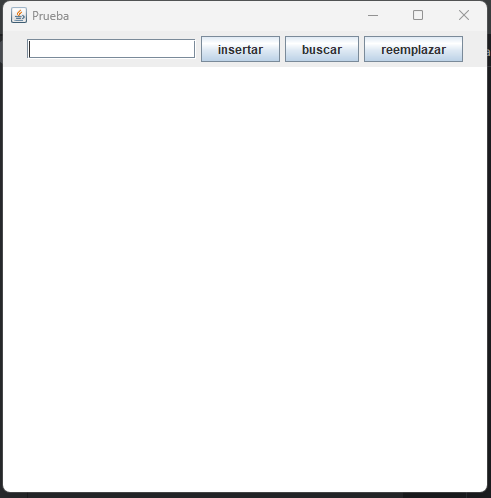
\includegraphics[width=0.8\textwidth,keepaspectratio]{img/pantallaInicial.png}\\
		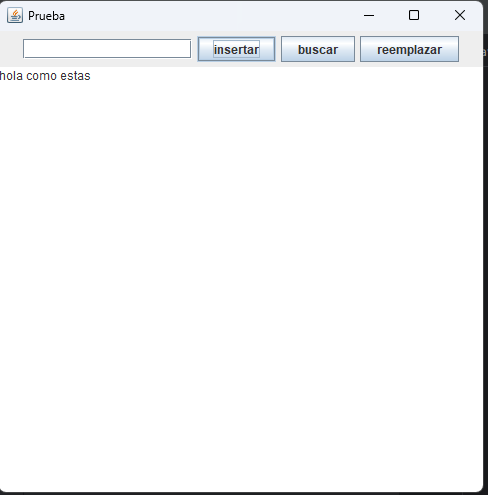
\includegraphics[width=0.8\textwidth,keepaspectratio]{img/insertandoOracion.png}\\
		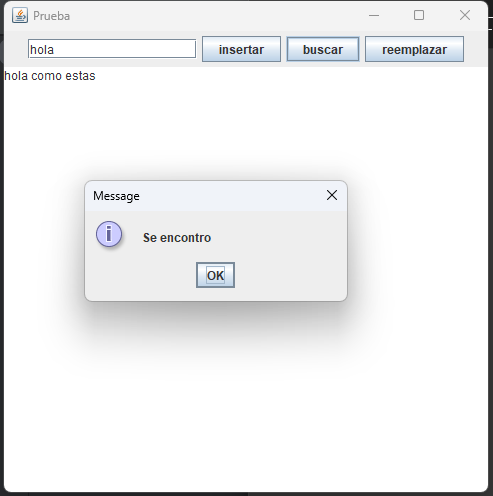
\includegraphics[width=0.8\textwidth,keepaspectratio]{img/buscandoPalabra.png}\\
		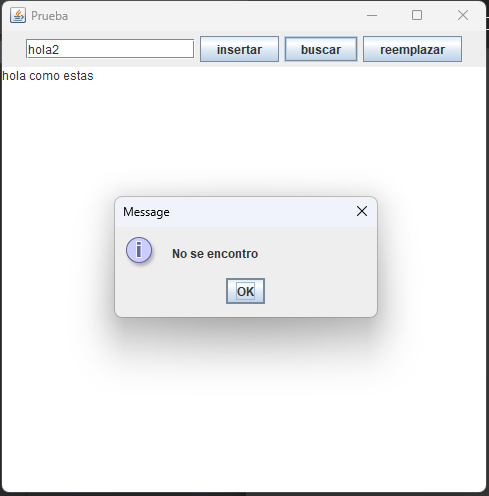
\includegraphics[width=0.8\textwidth,keepaspectratio]{img/buscandoPalabra2.png}\\
		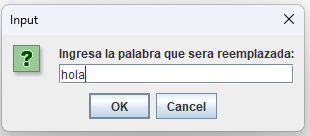
\includegraphics[width=0.8\textwidth,keepaspectratio]{img/reemplazando1.png}\\
		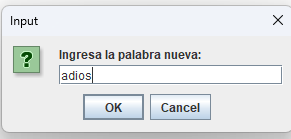
\includegraphics[width=0.8\textwidth,keepaspectratio]{img/reemplazando2.png}\\
		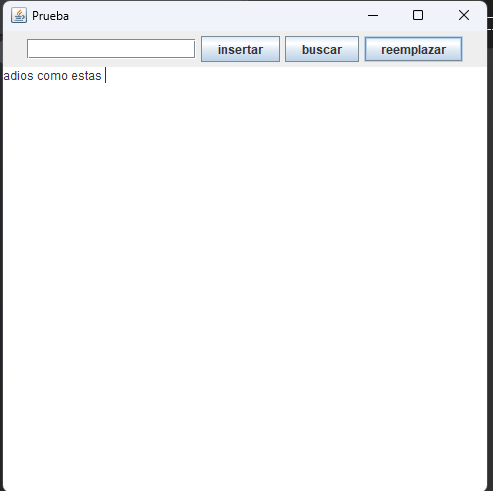
\includegraphics[width=0.8\textwidth,keepaspectratio]{img/reemplazo.png}\\
		\textbf{Cuestionario.}  \\
		\textbf{¿Cómo se utiliza esta estructura de datos para almacenar prefijos?.}  \\
		\textbf{ En un Trie, cada nodo representa un carácter y las rutas desde la raíz hasta los nodos hoja forman palabras o cadenas completas. Esto permite una búsqueda eficiente de palabras que comparten un mismo prefijo.}\\
		\textbf{¿Cómo realizó la funcionalidad de reemplazar texto?.}  \\
		La opción de reemplazar se aplica sobre palabras individuales, al ingresar una palabra para reemplazar por otra primero se evalúa la existencia de la palabra en el ArrayList de palabras. En caso de encontrarla se procede a colocar la nueva palabra dentro de la posición de la antigua, posteriormente se procede a llamar a la función reemplazar del Trie, la cual elimina la palabra antigua e inserta la nueva palabra.\\
		\hline
		%%%%%%%%%%%%			
	\end{longtable}
	%%%%%%%%%%%%%%%%%%%%%%%%
	\begin{table}[H]
		\begin{tabular}{|p{15cm}|}
			\hline 
			\rowcolor{tablebackground}
			\color{white}\textbf{LECCIONES APRENDIDAS Y CONCLUSIONES}  \\
			\hline 
			\textbf{Se aprendio a como implementar los principales metodos de los Tries
			como lo son la insercion, busqueda y eliminacion. Al igual que hacer un recuerdo del uso
			de intefaces graficas.}\\
		\hline 
		%%%%%%%%%%%%
		\rowcolor{tablebackground}
		\color{white}\textbf{REFERENCIAS Y BIBLIOGRAFÍA}  \\
		\hline 
		\textbf{[1]\url{https://es.wikipedia.org/wiki/Trie}}\\
		\hline 
		%%%%%%%%%%%%			
	\end{tabular}
\end{table}
%%%%%%%%%%%%%%%%%%%%%%%%
\end{document}
